\documentclass[12pt,twoside]{article}
\usepackage{jmlda}
%\NOREVIEWERNOTES
\title
    [Образец оформления статьи для публикации] % Краткое название; не нужно, если полное название влезает в~колонтитул
    {Образец оформления статьи для публикации в журнале <<Машинное обучение и анализ данных>>: файл jmlda-example.tex}
\author
    [Автор~И.\,О.] % список авторов для колонтитула; не нужен, если основной список влезает в колонтитул
    {Автор~И.\,О., Соавтор~И.\,О., Фамилия~И.\,О.} % основной список авторов, выводимый в оглавление
    [Автор~И.\,О.$^1$, Соавтор~И.\,О.$^2$, Фамилия~И.\,О.$^2$] % список авторов, выводимый в заголовок; не нужен, если он не отличается от основного
\thanks
    {Работа выполнена при финансовой поддержке РФФИ, проект \No\,00-00-00000.
   Научный руководитель:  Стрижов~В.\,В.
   Задачу поставил:  Эксперт~И.\,О.
    Консультант:  Консультант~И.\,О.}
\email
    {author@site.ru}
\organization
    {$^1$Организация; $^2$Организация}
\abstract
    {Данный текст является образцом оформления статьи, подаваемой для публикации в журнале <<Машинное обучение и анализ данных>>.
    Аннотация кратко характеризует основную цель работы,
    особенности предлагаемого подхода и~основные результаты.

\bigskip
\textbf{Ключевые слова}: \emph {ключевое слово, ключевое слово,
еще ключевые слова}.}
\titleEng
    {JMLDA paper example: file jmlda-example.tex}
\authorEng
    {Author~F.\,S.$^1$, CoAuthor~F.\,S.$^2$, Name~F.\,S.$^2$}
\organizationEng
    {$^1$Organization; $^2$Organization}
\abstractEng
    {This document is an example of paper prepared with \LaTeXe\
    typesetting system and style file \texttt{jmlda.sty}.

    \bigskip
    \textbf{Keywords}: \emph{keyword, keyword, more keywords}.}
\begin{document}
\maketitle
%\linenumbers
\section{Введение}
После аннотации, но перед первым разделом,
располагается введение, включающее в себя
описание предметной области,
обоснование актуальности задачи,
краткий обзор известных результатов,
и~т.\,п~\cite{author09anyscience,myHandbook,author09first-word-of-the-title,voron06latex,author-and-co2007,Lvovsky03}.

\section{Название раздела}
Данный документ демонстрирует оформление статьи,
подаваемой в электронную систему подачи статей \url{http://jmlda.org/papers} для публикации в журнале <<Машинной обучение и анализ данных>>.
Более подробные инструкции по~стилевому файлу \texttt{jmlda.sty}
и~использованию издательской системы \LaTeXe\
находятся в~документе \texttt{authors-guide.pdf}.
Работу над статьёй удобно начинать с~правки \TeX-файла данного документа.

\paragraph{Название параграфа.}
%Первый раздел может содержать формальную постановку задачи,
%основные определения и~обозначения,
%известные факты, необходимые для понимания основных результатов работы,
%и~т.\,п.
Нет ограничений на~количество разделов и~параграфов в~статье.
Разделы и~параграфы не~нумеруются.

\paragraph{Теоретическую часть работы} желательно структурировать
с~помощью окружений
Def, Axiom, Hypothesis, Problem, Lemma, Theorem, Corollary, State, Example, Remark.

\begin{Def}
    Математический текст \emph{хорошо структурирован},
    если в~нём выделены определения, теоремы, утверждения, примеры, и~т.\,д.,
    а~неформальные рассуждения (мотивации, интерпретации)
    вынесены в~отдельные параграфы.
\end{Def}

\begin{State}
    Мотивации и~интерпретации наиболее важны для понимания сути работы.
\end{State}

\begin{Theorem}
    Не~менее $90\%$ коллег, заинтересовавшихся Вашей статьёй,
    прочитают в~ней не~более~$10\%$ текста.
\end{Theorem}

\begin{Proof}
    Причём это будут именно те~разделы, которые не содержат формул.
\end{Proof}

\begin{Remark}
    Выше показано применение окружений
    Def, Theorem, State, Remark, Proof.
\end{Remark}

\section{Некоторые формулы}

Образец формулы: $f(x_i,\alpha^\gamma)$.

Образец выключной формулы без номера:
\[
    y(x,\alpha) =
    \begin{cases}
        -1, & \text{если } f(x,\alpha)<0;  \\
        +1, & \text{если } f(x,\alpha)\geq 0.
    \end{cases}
\]

Образец выключной формулы с номером:
\begin{equation}
\label{eq:cases}
    y(x,\alpha) =
    \begin{cases}
        -1, & \text{если } f(x,\alpha)<0;  \\
        +1, & \text{если } f(x,\alpha)\geq 0.
    \end{cases}
\end{equation}

Образец выключной формулы, разбитой на две строки с~помощью окружения align:
\begin{align}
    R'_N(F)
        = \frac1N \sum_{i=1}^N
        \Bigl(
            & P(+1\cond x_i) C\bigl(+1,F(x_i)\bigr)+{}
        \notag % подавили номер у первой строки
    \\ {}+{}
            & P(-1\cond x_i) C\bigl(-1,F(x_i)\bigr)
        \Bigr).
        \label{eq:R(F)}
\end{align}

Образцы ссылок: формулы~\eqref{eq:cases} и~\eqref{eq:R(F)}.

\section{Пример илюстрации}

Рисунки вставляются командой \verb|\includegraphics|,
желательно с~выравниванием по~ширине колонки: \verb|[width=\linewidth]|.

Практически все популярные пакеты рисуют графики с подписями, которые трудно читать на бумаге и на слайдах из-за малого размера шрифта. Шрифт на графиках (подписи осей и цифры на осях) должны быть такого же размера, что и основной текст.

\begin{figure}[h]
  \subfloat[Первый рисунок]{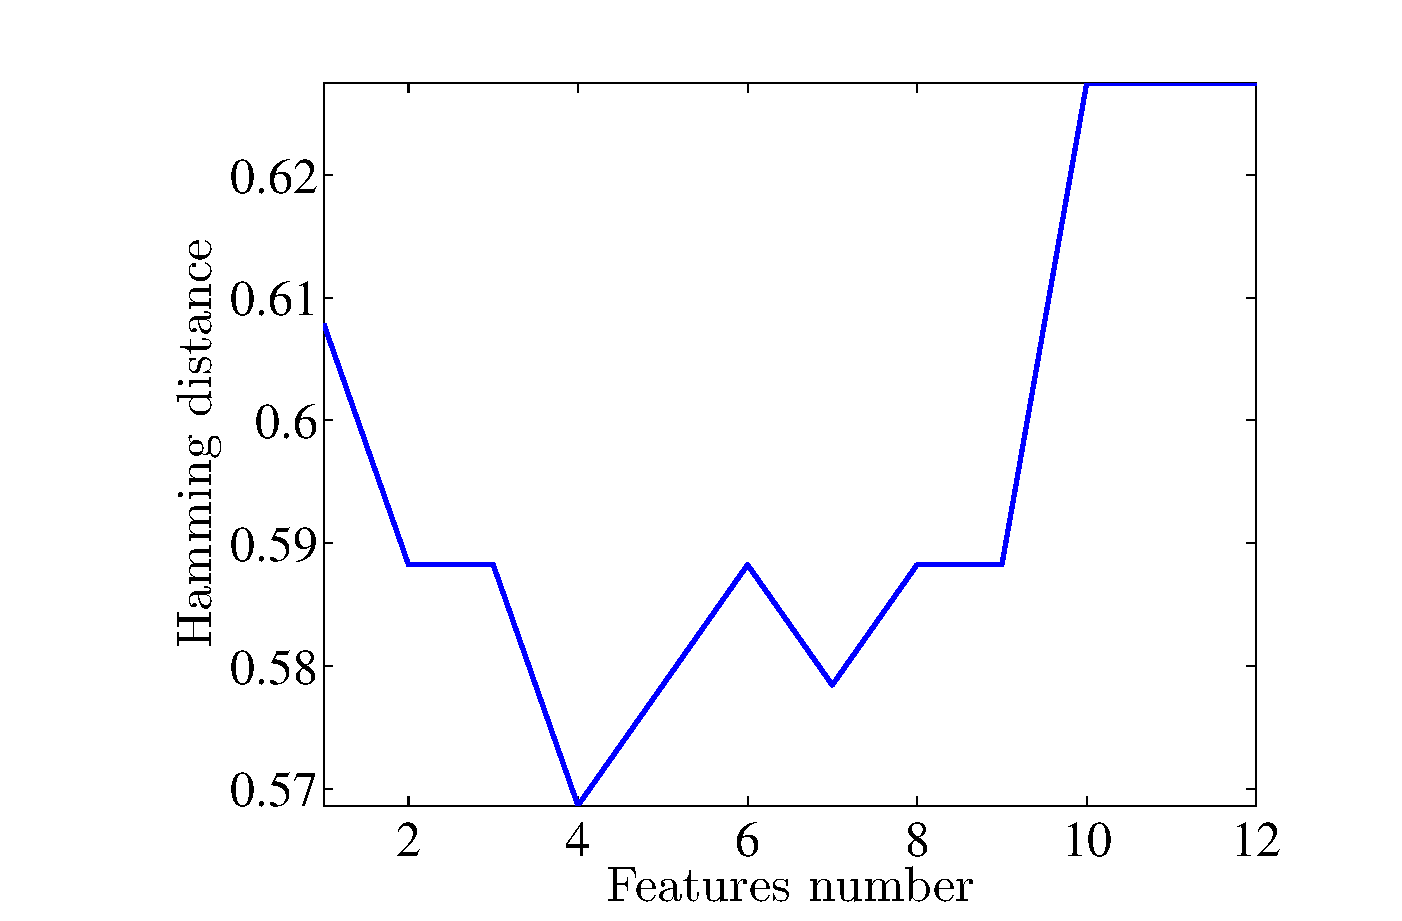
\includegraphics[width=0.5\textwidth]{figExample1}}
  \subfloat[Второй рисунок]{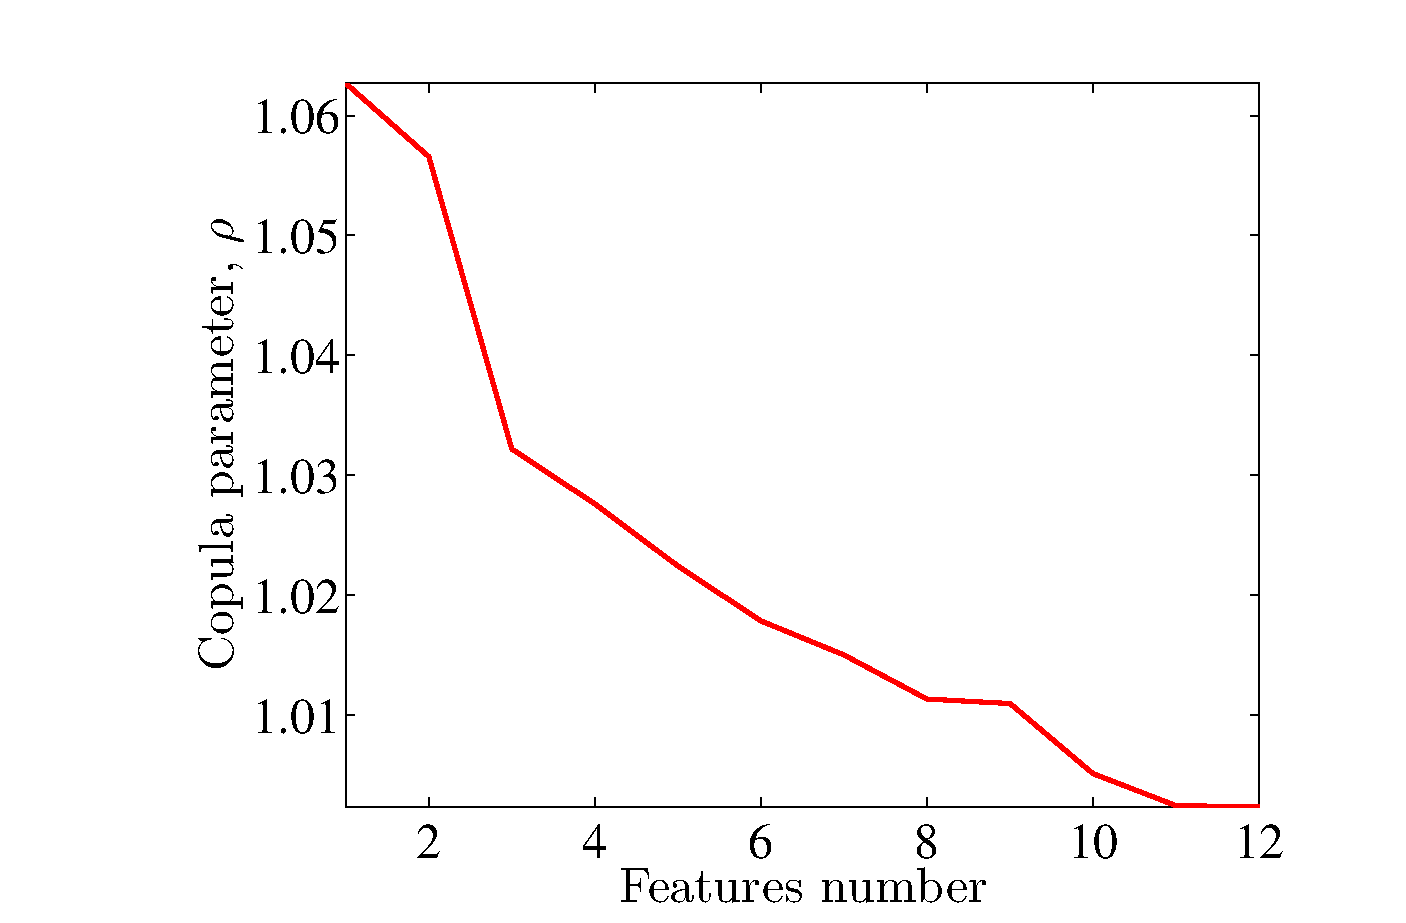
\includegraphics[width=0.5\textwidth]{figExample2}}\\
\caption{Подпись должна размещаться под рисунком. }
\label{fg:Example}
\end{figure}

При значительном количестве рисунков рекомендуется группировать иx в одном окружении \verb|{figure}|, как это сделано на рис.~\ref{fg:Example}.

\section{Пример таблицы}
Подпись делается \emph{над таблицей}, см.~таблицу~\ref{TabExample}.


\begin{table}[t]%\small
    \caption{Подпись размещается над таблицей.}
    \label{TabExample}
    \centering\medskip%\tabcolsep=2pt%\small
    \begin{tabular}{lrrr}
    \headline
        Задача
            & \multicolumn{1}{c}{CCEL}
            & \multicolumn{1}{c}{boosting} \\
    \headline
        {\tt Cancer}
            & $\mathbf{3.46}  \pm 0.37$ (3.16)
            & $4.14 \pm 1.48$ \\
        {\tt German}
            & $\mathbf{25.78} \pm 0.65$ (1.74)
            & $29.48 \pm 0.93$ \\
        {\tt Hepatitis}
            & $18.38 \pm 1.43$ (2.87)
            & $19.90 \pm 1.80$ \\
    \hline
    \end{tabular}
\end{table}

\section{Заключение}
Желательно, чтобы этот раздел был, причём он не~должен дословно повторять аннотацию.
Обычно здесь отмечают,
каких результатов удалось добиться,
какие проблемы остались открытыми.


\bibliographystyle{unsrt}
\bibliography{jmlda-bib}
%\begin{thebibliography}{1}

%\bibitem{author09anyscience}
%    \BibAuthor{Author\;N.}
%    \BibTitle{Paper title}~//
%    \BibJournal{10-th Int'l. Conf. on Anyscience}, 2009.  Vol.\,11, No.\,1.  Pp.\,111--122.
%\bibitem{myHandbook}
%    \BibAuthor{Автор\;И.\,О.}
%    Название книги.
%    Город: Издательство, 2009. 314~с.
%\bibitem{author09first-word-of-the-title}
%    \BibAuthor{Автор\;И.\,О.}
%    \BibTitle{Название статьи}~//
%    \BibJournal{Название конференции или сборника},
%    Город:~Изд-во, 2009.  С.\,5--6.
%\bibitem{author-and-co2007}
%    \BibAuthor{Автор\;И.\,О., Соавтор\;И.\,О.}
%    \BibTitle{Название статьи}~//
%    \BibJournal{Название журнала}. 2007. Т.\,38, \No\,5. С.\,54--62.
%\bibitem{bibUsefulUrl}
%    \BibUrl{www.site.ru}~---
%    Название сайта.  2007.
%\bibitem{voron06latex}
%    \BibAuthor{Воронцов~К.\,В.}
%    \LaTeXe\ в~примерах.
%    2006.
%    \BibUrl{http://www.ccas.ru/voron/latex.html}.
%\bibitem{Lvovsky03}
%    \BibAuthor{Львовский~С.\,М.} Набор и вёрстка в пакете~\LaTeX.
%    3-е издание.
%    Москва:~МЦHМО, 2003.  448~с.
%\end{thebibliography}

% Решение Программного Комитета:
%\ACCEPTNOTE
%\AMENDNOTE
%\REJECTNOTE
\end{document}
